%-----------------------------------LICENSE------------------------------------%
%   This file is part of tikz_figures.                                         %
%                                                                              %
%   tikz_figures is free software: you can redistribute it and/or              %
%   modify it it under the terms of the GNU General Public License as          %
%   published by the Free Software Foundation, either version 3 of the         %
%   License, or (at your option) any later version.                            %
%                                                                              %
%   tikz_figures is distributed in the hope that it will be useful,            %
%   but WITHOUT ANY WARRANTY; without even the implied warranty of             %
%   MERCHANTABILITY or FITNESS FOR A PARTICULAR PURPOSE.  See the              %
%   GNU General Public License for more details.                               %
%                                                                              %
%   You should have received a copy of the GNU General Public License along    %
%   with tikz_figures.  If not, see <https://www.gnu.org/licenses/>.           %
%------------------------------------------------------------------------------%

% Use the standalone class for displaying the tikz image on a small PDF.
\documentclass[crop, tikz]{standalone}

% Import the tikz package to use for the drawing.
\usepackage{tikz}

% Begin the document.
\begin{document}

    % Draw the figure.
    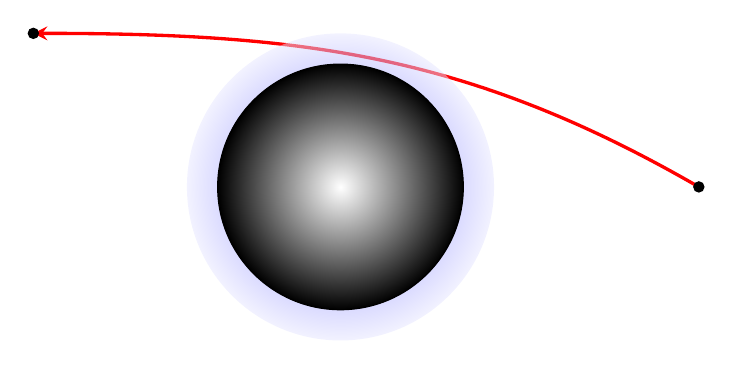
\begin{tikzpicture}[%
        line cap = round,
        > = stealth,
        scale = 1.3
    ]

        % Coordinates for the start and end points of the line, and the origin.
        \coordinate (A) at (3.5, 0.0);
        \coordinate (B) at (-3.0, 1.5);
        \coordinate (O) at (0.0, 0.0);

        % Draw curved thick red line from A to B.
        \draw[draw=red, ->, very thick] (A) to[in = 0, out = 150] (B);

        % Draw transparent "atmosphere" shaded light blue.
        \draw[%
            draw = none,
            inner color = blue,
            outer color = blue!10!white,
            opacity=0.5
        ] (O) circle (15.0mm) (O) circle (1.2cm);

        % Draw a ball on top of the atmosphere representing a planet.
        \draw[%
            inner color = white,
            outer color = black!100!gray
        ] (O) circle (1.2cm);

        % Add dots at the points A and B.
        \draw[fill = black] (A) circle (0.5mm);
        \draw[fill = black] (B) circle (0.5mm);
    \end{tikzpicture}
\end{document}
